\documentclass[17pt,xcolor=x11names]{beamer}
\usepackage[utf8]{inputenc}

\usepackage{tikz, tikz-3dplot}

%\usepackage{tkz-graph}

\usetikzlibrary{arrows,calc,automata,chains,matrix,positioning,scopes,decorations.pathmorphing,decorations.markings, shapes.misc,decorations.pathreplacing}

\tikzset{cross/.style={cross out, draw=black, minimum size=2*(#1-\pgflinewidth), inner sep=0pt, outer sep=0pt},
%default radius will be 1pt. 
cross/.default={2pt}}

\usecolortheme{seagull}
\useoutertheme{infolines}
\usefonttheme[onlymath]{serif}

\setbeamertemplate{headline}[default]
\setbeamertemplate{navigation symbols}{}
\mode<beamer>{\setbeamertemplate{blocks}[rounded][shadow=true]}
\setbeamercovered{transparent}
\setbeamercolor{block body example}{fg=blue, bg=black!20}

\newcommand\undermat[2]{%
  \makebox[0pt][l]{$\smash{\underbrace{\phantom{%
    \begin{matrix}#2\end{matrix}}}_{\text{$#1$}}}$}#2}

\title[Nézőponthelyreállítás]{Nézőponthelyreállítás több kameraképből}
\subtitle{}
\author[Kriván Bálint]{\textbf{Kriván Bálint} (\texttt{CBVOEN})\\[10pt]
\footnotesize Dr. Kovács Gábor (\texttt{kovacsg@tmit.bme.hu})}
\institute[BME]{}
\date{2014. dec. 16.}

\begin{document}

\begin{frame}\maketitle\end{frame}

\begin{frame}{Feladat}
\begin{itemize}
\item \textbf{Nézőponthelyreállítás} \\\vspace{10pt}
\item szinkronizáció, kalibráció
\item objektum-detekció
\item rekonstrukció
\item közös koordináta-rendszer
\item kontúr rajzolás
\end{itemize}
\end{frame}

\begin{frame}{Szinkronizáció}
\begin{itemize}
\item időbélyeg
\item trigger-esemény
\begin{itemize}
\item \textit{clapperboard}
\item \textbf{lézerpont detekció} $\rightarrow$ Önálló labor. 1.
\end{itemize}
\end{itemize}
\end{frame}

\begin{frame}{Objektum-detekció}
\begin{itemize}
\item előtér-háttér modell építés
\end{itemize}
\begin{center}
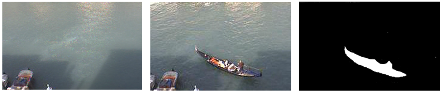
\includegraphics[width=330pt]{figures/mog.png}
\end{center}
\begin{itemize}
\item \textcolor{gray}{optikai-folyamok (később)}
\end{itemize}
\end{frame}

\begin{frame}{Sztereó-látás 1.}
\begin{itemize}
\item páronként kalibrálunk
\item rektifikáció
\item elmozdulás a két képen $\rightarrow$ mélység
\end{itemize}
\begin{center}
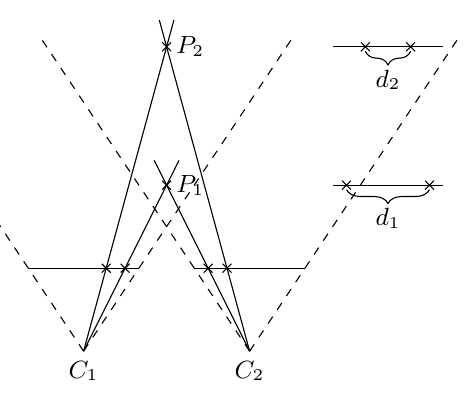
\begin{tikzpicture}[x=20,y=20]
    \tikzstyle{every node}=[font=\small]
\tikzset{
    position label/.style={
       below = 3pt,
       text height = 1.5ex,
       text depth = 1ex
    },
   brace/.style={
     decoration={brace,amplitude=5pt},
     decorate
   }
}
  \coordinate (L1) at (0, 0);
  \coordinate (L2) at (2, 0);
  \draw (L1) -- (L2);
  
  \coordinate (C1) at (1, -1.5);
  \node [below] at (C1) {$C_1$};

  \draw [dashed, shorten >= -100pt] (C1) -- (L1);
  \draw [dashed, shorten >= -100pt] (C1) -- (L2);

  
  \coordinate (R1) at (3, 0);
  \coordinate (R2) at (5, 0);
  \draw (R1) -- (R2);
  
  \coordinate (C2) at (4, -1.5);
  \node [below] at (C2) {$C_2$};

  \draw [dashed, shorten >= -100pt] (C2) -- (R1);
  \draw [dashed, shorten >= -100pt] (C2) -- (R2);

  \coordinate (P1) at (2.5, 1.5);
  \node [cross] at (P1) {};
  \node [right] at (P1) {$P_1$};
  
  \coordinate (P2) at (2.5, 4);
  \node [cross] at (P2) {};
  \node [right] at (P2) {$P_2$};

  \draw [shorten >= -10pt] (C1) -- (P1);
  \draw [shorten >= -10pt] (C1) -- (P2);
  \draw [shorten >= -10pt] (C2) -- (P1);
  \draw [shorten >= -10pt] (C2) -- (P2);
  
  \coordinate (P2B) at (1.4090, 0);
  \node [cross] at (P2B) {};
  \node [above left] at (P2B) {};
  
  \coordinate (P1B) at (1.75, 0);
  \node [cross] at (P1B) {};
  \node [above right] at (P1B) {};
  
  \coordinate (P2J) at (3.591, 0);
  \node [cross] at (P2J) {};
  \node [above right] at (P2J) {};
  
  \coordinate (P1J) at (3.25, 0);
  \node [cross] at (P1J) {};
  \node [above left] at (P1J) {};
  
  % távolságok másolata
  
  \draw (5.5, 4) -- (7.5, 4);
  \node [cross] (T1) at (6.9090, 4) {};
  \node [cross] (T2) at (6.091, 4) {};
  \draw (5.5, 1.5) -- (7.5, 1.5);
  \node [cross] (B1) at (7.25, 1.5) {};
  \node [cross] (B2) at (5.75, 1.5) {};
  
   \draw [brace] (T1.south) -- (T2.south) node [position label, pos=0.5] {$d_2$};
   \draw [brace] (B1.south) -- (B2.south) node [position label, pos=0.5] {$d_1$};
  
\end{tikzpicture}
\end{center}
\end{frame}

\begin{frame}{Sztereó-látás 2.}
\begin{center}
  \begin{tikzpicture}[x=300,y=330]
	\node[anchor=south west,inner sep=0] at (0.51,0) {
\includegraphics[width=150pt] {figures/disparity_sgbm.jpg}};
    \node[anchor=south west,inner sep=0] at (0,0) {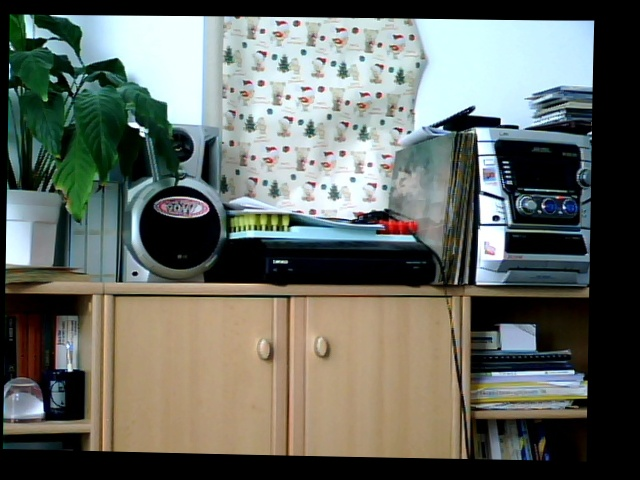
\includegraphics[width=150pt]    {figures/left01_mapped.jpg}};
\end{tikzpicture}
\end{center}
\end{frame}

\begin{frame}{Optikai-folyamok 1.}
\begin{itemize}
\item minden kamera egyénileg rekonstruál
\item optikai-folyamok $\rightarrow$ egyező pontok
\item háromszögelés $\rightarrow$ objektum struktúrája
\end{itemize}
\end{frame}

\begin{frame}{Optikai-folyamok 2.}
\begin{itemize}
\item Färneback: sűrű optikai-folyam
\end{itemize}
\begin{center}
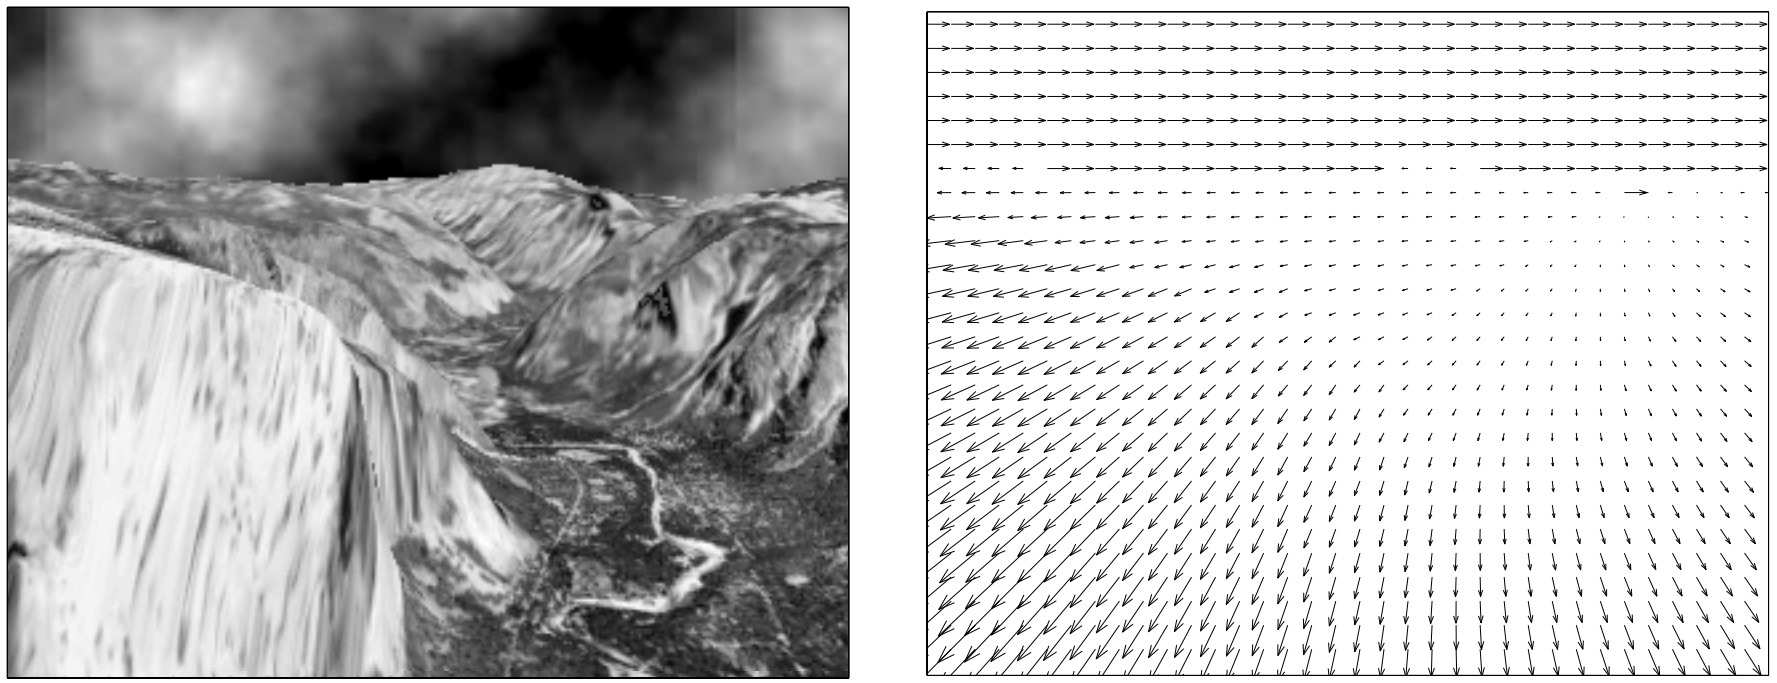
\includegraphics[width=330pt]{figures/farneback.png}
\end{center}
\end{frame}

\begin{frame}{Optikai-folyamok 3.}
\begin{itemize}
\item háromszögelés
\end{itemize}
\begin{center}
\tdplotsetmaincoords{60}{130}
\begin{tikzpicture}[scale=0.9,line join = round, line cap = round, >=triangle 45, tdplot_main_coords]
  
  \coordinate (O) at (0, 0, 0);
  
  % kocka
  
  \coordinate (C1) at (-4.5, -2, 1);
  \coordinate (C2) at (-4.5, -1, 1);
  \coordinate (C3) at (-4.5, -1, 2);
  \coordinate (C4) at (-4.5, -2, 2);
  \coordinate (C1B) at (-5, -2, 1);
  \coordinate (C2B) at (-5, -1, 1);
  \coordinate (C3B) at (-5, -1, 2);
  \coordinate (C4B) at (-5, -2, 2);
    \node [below right] at (C2) {\small $(X, Y, Z)$};

  \draw [dashed] (C1) -- (C2);
  \draw [dashed] (C2) -- (C3);
  \draw [dashed] (C3) -- (C4);
  \draw [dashed] (C4) -- (C1);
  \draw [dashed] (C1) -- (C1B);
  \draw [dashed] (C2) -- (C2B);
  \draw [dashed] (C3) -- (C3B);
  \draw [dashed] (C4) -- (C4B);
  \draw [dashed] (C1B) -- (C2B);
  \draw [dashed] (C2B) -- (C3B);
  \draw [dashed] (C3B) -- (C4B);
  \draw [dashed] (C4B) -- (C1B);
  
  
  % képsík
  
  \coordinate (I1) at (0, 0, 0);
  \coordinate (I2) at (0, 4, 0);
  \coordinate (I3) at (0, 4, 3);
  \coordinate (I4) at (0, 0, 3);

  \coordinate (_I1) at (-0.7, 5, 0);
  \coordinate (_I2) at (-0.7, 5, 3);
  \coordinate (_I3) at (-4.7, 5, 3);
  \coordinate (_I4) at (-4.7, 5, 0);


  \draw (I1) -- (I2);
  \draw (I2) -- (I3);
  \draw (I3) -- (I4);
  \draw (I4) -- (I1);
  
  \draw (_I1) -- (_I2);
  \draw (_I2) -- (_I3);
  \draw (_I3) -- (_I4);
  \draw (_I4) -- (_I1);

  \coordinate (UV) at (0, 0.421, 1.2368);
  \node [cross] at (UV) {};

  \coordinate (UV2) at (-3.5182, 5, 1.2727);
  \node [cross] at (UV2) {};

  % optikai tengely
  \coordinate (P1) at (0, 2, 1.5);
  \coordinate (C1) at (5, 2, 1.5);
  \coordinate (A1) at (-1, 2, 1.5);

  \coordinate (P2) at (-2.7, 5, 1.5);
  \coordinate (C2_) at (-2.7, 10, 1.5);
  \coordinate (A2) at (-2.7, 4, 1.5);

  \node [below] at (C1) {\small $C_1$};
  \node [below] at (C2_) {\small $C_2$};
  \draw (C1) -- (P1);
  \draw (C2_) -- (P2);
  \node [cross] at (P1) {};
  \node [cross] at (P2) {};
  \node [below right] at (P1) {};
  \node [below left] at (P2) {};
  \draw [dashed,-latex] (P1) -- (A1);
  \draw [dashed,-latex] (P2) -- (A2);
  
  % leképezés
  
  \draw [dotted] (C1) -- (C2);
  \draw [dotted] (C2_) -- (C2);
  
\end{tikzpicture}
\end{center}
\end{frame}

\begin{frame}{Két eljárás közös része}
\begin{itemize}
\item közös koordináta-rendszerbe transzformáció
\item kontúr-rajzolás\\\vspace{30pt}
\item következő képkocka$\ldots$
\end{itemize}
\end{frame}

\begin{frame}{Összefoglalás, következő félév}
\begin{itemize}
\item irodalomkutatás, elméleti háttér
\item 2 rekonstrukciós eljárás kidolgozása\\\vspace{20pt}
\item elkezdett implementáció folytatása
\item tesztelés, értékelés
\end{itemize}
\end{frame}

\end{document}
